%%%%%%%%%%%%%%%%%%%%%%%%%%%%%%%%%%%%
%                                  %
% Titre  : s_f.tex                 %
% Sujet  : Manuel de l'utilisateur %
%          du projet 'Scotch'      %
%          Formats de fichiers 6.0 %
% Auteur : Francois Pellegrini     %
%                                  %
%%%%%%%%%%%%%%%%%%%%%%%%%%%%%%%%%%%%

\section{Files and data structures}
\label{sec-file}

For the sake of portability, readability, and reduction of storage space,
all the data files shared by the different programs of the
\scotch\ project are coded in plain ASCII text exclusively.
Although we may speak of ``lines'' when describing file formats,
text-formatting characters such as newlines or tabulations are not
mandatory, and are not taken into account when files are read.
They are only used to provide better readability and understanding.
Whenever numbers are used to label objects, and unless explicitely
stated, \textbf{numberings always start from zero}, not one.

\subsection{Graph files}
\label{sec-file-sgraph}

Graph files, which usually end in ``\texttt{\@.grf}'' or
``\texttt{\@.src}'', describe valuated graphs, which can be valuated
process graphs to be mapped onto target architectures, or graphs
representing the adjacency structures of matrices to order.

Graphs are represented by means of adjacency lists: the definition
of each vertex is accompanied by the list of all of its neighbors, i.e.
all of its adjacent arcs. Therefore, the overall number of edge data is
twice the number of edges.
\\

Since version \textsc{3.3} has been introduced a new file format, referred
to as the ``new-style'' file format, which replaces the previous,
``old-style'', file format. The two advantages of the new-style
format over its predecessor are its greater compacity, which results
in shorter I/O times, and its ability to handle easily graphs output
by C or by Fortran programs.

Starting from version \textsc{4.0}, only the new format is supported. To
convert remaining old-style graph files into new-style graph files,
one should get version \textsc{3.4} of the \scotch\ distribution, which
comprises the \texttt{scv} file converter, and use it to produce
new-style \scotch\ graph files from the old-style \scotch\ graph files
which it is able to read. See section~\ref{sec-prog-gcv} for a
description of \texttt{gcv}, formerly called \texttt{scv}.
\\

The first line of a graph file holds the graph file version number,
which is currently~\texttt{0}. The second line holds the number of
vertices of the graph (referred to as \texttt{vertnbr} in \libscotch; see
for instance Figure~\ref{fig-lib-graf-one},
page~\pageref{fig-lib-graf-one}, for a detailed example), followed by
its number of arcs (unappropriately called \texttt{edgenbr}, as it is in
fact equal to twice the actual number of edges). The third line holds
two figures: the graph base index value (\texttt{baseval}), and a numeric
flag.

The graph base index value records the value of the starting index
used to describe the graph; it is usually $0$ when the graph has been
output by C programs, and $1$ for Fortran programs. Its purpose is to
ease the manipulation of graphs within each of these two environments,
while providing compatibility between them.

The numeric flag, similar to the one used by the \chaco\ graph
format~\cite{hele93c}, is made of three decimal digits.
A non-zero value in the units indicates that vertex weights are provided.
A non-zero value in the tenths indicates that edge weights are provided.
A non-zero value in the hundredths indicates that vertex labels are provided;
if it is the case, vertices can be stored in any order in the file; else,
natural order is assumed, starting from the graph base index.

This header data is then followed by as many lines as there are
vertices in the graph, that is, \texttt{vertnbr} lines. Each of these
lines begins with the vertex label, if necessary, the vertex load, if
necessary, and the vertex degree, followed by the description of the
arcs. An arc is defined by the load of the edge, if necessary, and by
the label of its other end vertex.
The arcs of a given vertex can be provided in any order in its
neighbor list. If vertex labels are provided, vertices can also be
stored in any order in the file.

Figure~\ref{fig-file-sgraph} shows the contents of a graph file
modeling a cube with unity vertex and edge weights and base $0$.

\begin{figure}[hbt]
\begin{center}
\begin{minipage}{7.3cm}
{\renewcommand{\baselinestretch}{1.05}
 \footnotesize \tt
\begin{verbatim}
0
8       24
0       000
3       4       2       1
3       5       3       0
3       6       0       3
3       7       1       2
3       0       6       5
3       1       7       4
3       2       4       7
3       3       5       6
\end{verbatim}}
\end{minipage}
\end{center}
\caption{Graph file representing a cube.}
\label{fig-file-sgraph}
\end{figure}

\subsection{Mesh files}
\label{sec-file-smesh}

Mesh files, which usually end in ``\texttt{\@.msh}'', describe valuated
meshes, made of elements and nodes, the elements of which can be
mapped onto target architectures, and the nodes of which can be
reordered.

Meshes are bipartite graphs, in the sense that every element is
connected to the nodes that it comprises, and every node is connected
to the elements to which it belongs. No edge connects any two element
vertices, nor any two node vertices.  One can also think of meshes as
hypergraphs, such that nodes are the vertices of the hypergraph and
elements are hyper-edges which connect multiple nodes, or reciprocally
such that elements are the vertices of the hypergraph and nodes are
hyper-edges which connect multiple elements.

Since meshes are graphs, the structure of mesh files resembles very
much the one of graph files described above in
section~\ref{sec-file-sgraph}, and differs only by its header, which
indicates which of the vertices are node vertices and element
vertices.
\\

The first line of a mesh file holds the mesh file version number,
which is currently~\texttt{1}. Graph and mesh version numbers will always
differ, which enables application programs to accept both file formats
and adapt their behavior according to the type of input data.  The
second line holds the number of elements of the mesh (\texttt{velmnbr}),
followed by its number of nodes (\texttt{vnodnbr}), and its overall
number of arcs (\texttt{edgenbr}, that is, twice the number of edges
which connect elements to nodes and vice-versa).

The third line holds three figures: the base index of the first
element vertex in memory (\texttt{velmbas}), the base index of the first
node vertex in memory (\texttt{vnodbas}), and a numeric flag.

The \scotch\ mesh file format requires that all nodes and all elements
be assigned to contiguous ranges of indices. Therefore, either all
element vertices are defined before all node vertices, or all node
vertices are defined before all element vertices. The node and element
base indices indicate at the same time whether elements or nodes are
put in the first place, as well as the value of the starting index
used to describe the graph. Indeed, if
$\mbox{\texttt{velm}}\-\mbox{\texttt{bas}} <
\mbox{\texttt{vnod}}\-\mbox{\texttt{bas}}$, then elements have the 
smallest indices, \texttt{velmbas} is the base value of the underlying
graph (that is, \texttt{baseval} = \texttt{velmbas}), and
$\mbox{\texttt{velmbas}} + \mbox{\texttt{velmnbr}} =
\mbox{\texttt{vnodbas}}$
holds. Conversely, if $\mbox{\texttt{velm}}\-\mbox{\texttt{bas}}
> \mbox{\texttt{vnod}}\-\mbox{\texttt{bas}}$, then nodes have the
smallest indices, \texttt{vnodbas} is the base value of the underlying
graph, (that is, \texttt{baseval} = \texttt{vnodbas}), and
$\mbox{\texttt{vnodbas}} + \mbox{\texttt{vnodnbr}} =
\mbox{\texttt{velmbas}}$ holds.

The numeric flag, similar to the one used by the \chaco\ graph
format~\cite{hele93c}, is made of three decimal digits.  A non-zero
value in the units indicates that vertex weights are provided.  A
non-zero value in the tenths indicates that edge weights are provided.
A non-zero value in the hundredths indicates that vertex labels are
provided; if it is the case, and if
$\mbox{\texttt{velm}}\-\mbox{\texttt{bas}} <
\mbox{\texttt{vnod}}\-\mbox{\texttt{bas}}$
(resp\@. $\mbox{\texttt{velm}}\-\mbox{\texttt{bas}} >
\mbox{\texttt{vnod}}\-\mbox{\texttt{bas}}$), the \texttt{velmnbr}
(resp\@. \texttt{vnodnbr}) first vertex lines are assumed to be element
(resp\@. node) vertices, irrespective of their vertex labels, and the
\texttt{vnodnbr} (resp\@. \texttt{velmnbr}) remaining vertex lines are
assumed to be node (resp\@. element) vertices; else, natural order is
assumed, starting at the underlying graph base index (\texttt{baseval}).

This header data is then followed by as many lines as there are
node and element vertices in the graph. These lines are similar
to the ones of the graph format, except that, in order to save
disk space, the numberings of nodes and elements all start from
the same base value, that is,
$\min(\mbox{\texttt{velm}}\-\mbox{\texttt{bas}},
\mbox{\texttt{vnod}}\-\mbox{\texttt{bas}})$ (also called
\texttt{baseval}, like for regular graphs).

For example, Figure~\ref{fig-file-smesh} shows the contents of the
mesh file modeling three square elements, with unity vertex and edge
weights, elements defined before nodes, and numbering of the
underlying graph starting from $1$. In memory, the three elements are
labeled from $1$ to $3$, and the eight nodes are labeled from $4$ to
$11$. In the file, the three elements are still labeled from $1$ to $3$,
while the eight nodes are labeled from $1$ to $8$.

When labels are used, elements and nodes may have similar labels,
but not two elements, nor two nodes, should have the same labels.

\begin{figure}[hbt]
\begin{center}
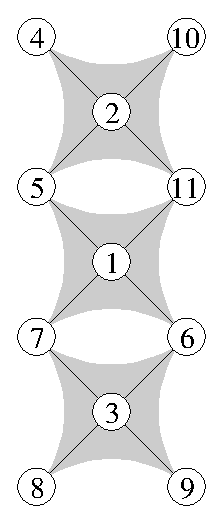
\includegraphics[scale=0.65]{s_f_msf.eps}
\hfil ~\hfil
\begin{minipage}[b]{7cm}
\verb+1+

\noi
\verb+3       8       24+

\noi
\verb+1       4       000+

\verb+4       2 +\makebox[0em][l]{\tiny (= 5)}\verb+      8 +\makebox[0em][l]{\tiny (= 11)}\verb+      4 +\makebox[0em][l]{\tiny (= 7)}\verb+      3 +\makebox[0em][l]{\tiny (= 6)}

\noi
\verb+4       7 +\makebox[0em][l]{\tiny (= 10)}\verb+      2 +\makebox[0em][l]{\tiny (= 5)}\verb+      8 +\makebox[0em][l]{\tiny (= 11)}\verb+      1 +\makebox[0em][l]{\tiny (= 4)}

\noi
\verb+4       5 +\makebox[0em][l]{\tiny (= 8)}\verb+      6 +\makebox[0em][l]{\tiny (= 9)}\verb+      3 +\makebox[0em][l]{\tiny (= 6)}\verb+      4 +\makebox[0em][l]{\tiny (= 7)}

\noi
\verb+1       2+

\noi
\verb+2       2       1+

\noi
\verb+2       1       3+

\noi
\verb+2       1       3+

\noi
\verb+1       3+

\noi
\verb+1       3+

\noi
\verb+1       2+

\noi
\verb+2       2       1+
%\begin{verbatim}
%1
%3       8       24
%1       4       000
%4       5       11      7       6
%4       10      5       11      4
%4       8       9       6       7
%1       2
%2       2       1
%2       1       3
%2       1       3
%1       3
%1       3
%1       2
%2       2       1
%\end{verbatim}
\end{minipage}
\end{center}
\caption{Mesh file representing three square elements, with unity
vertex and edge weights. Elements are defined before nodes, and
numbering of the underlying graph starts from $1$. The left part of
the figure shows the mesh representation in memory, with consecutive
element and node indices. The right part of the figure shows the
contents of the file, with both element and node numberings starting
from $1$, the minimum of the element and node base values.
Corresponding node indices in memory are shown in parentheses for the
sake of comprehension.}
\label{fig-file-smesh}
\end{figure}

\subsection{Geometry files}
\label{sec-file-geom}

Geometry files, which usually end in ``\texttt{\@.xyz}'', hold the coordinates
of the vertices of their associated graph or mesh.
These files are not used in the mapping process itself, since only
topological properties are taken into account then (mappings are
computed regardless of graph geometry).
They are used by visualization programs to compute
graphical representations of mapping results.

The first string to appear in a geometry file codes for its type, or
dimensionality. It is ``\texttt{1}'' if the file contains unidimensional
coordinates, ``\texttt{2}'' for bidimensional coordinates, and ``\texttt{3}'' for
tridimensional coordinates.
It is followed by the number of coordinate data stored in the file, which
should be at least equal to the number of vertices of the associated graph
or mesh, and by that many coordinate lines.
Each coordinate line holds the label of the vertex, plus one, two or three
real numbers which are the (X), (X,Y), or (X,Y,Z), coordinates of the graph
vertices, according to the graph dimensionality.
\\
Vertices can be stored in any order in the file. Moreover, a geometry
file can have more coordinate data than there are vertices in the
associated graph or mesh file; only coordinates the labels of which
match labels of graph or mesh vertices will be taken into account.
This feature allows all subgraphs of a given graph or mesh to share the
same geometry file, provided that graph vertex labels remain unchanged.
For example, Figure~\ref{fig-file-geom} shows the contents of the 3D~geometry
file associated with the graph of Figure~\ref{fig-file-sgraph}.
\begin{figure}[hbt]
\begin{center}
\begin{minipage}{4.6cm}
{\renewcommand{\baselinestretch}{1.05}
 \footnotesize \tt
\begin{verbatim}
3
8
0       0.0     0.0     0.0
1       0.0     0.0     1.0
2       0.0     1.0     0.0
3       0.0     1.0     1.0
4       1.0     0.0     0.0
5       1.0     0.0     1.0
6       1.0     1.0     0.0
7       1.0     1.0     1.0
\end{verbatim}
}\end{minipage}
\end{center}
\caption{Geometry file associated with the graph file of
         Figure~\protect\ref{fig-file-sgraph}.}
\label{fig-file-geom}
\end{figure}

\subsection{Target files}
\label{sec-file-target}

Target files describe the architectures onto which source graphs are mapped.
Instead of containing the structure of the target graph itself, as source
graph files do, target files define how target graphs are bipartitioned and
give the distances between all pairs of vertices (that is, processors).
Keeping the bipartitioning information within target files avoids
recomputing it every time a target architecture is used.
We are allowed to do so because, in our approach, the recursive
bipartitioning of the target graph is fully independent with respect to that
of the source graph (however, the opposite is false).

For space and time saving issues, some classical homogeneous architectures
(2D and 3D meshes and tori, hypercubes, complete graphs, etc\@.) have been
algorithmically coded within the mapper itself by the means of built-in
functions.
Instead of containing the whole graph decomposition data, their target
files hold only a few values, used as parameters by the built-in functions.

\subsubsection{Decomposition-defined architecture files}
\label{sec-file-target-deco}

Decomposition-defined architecture files are the way to describe
irregular target architectures that cannot be represented as
algorithmically-coded architectures.

Two main file formats coexist~: the ``\texttt{deco 0}'' and
``\texttt{deco 2}'' formats. ``\texttt{deco}'' stands for
``decomposition-defined architecture'', followed by the format
number. The ``\texttt{deco 1}'' format is a compiled form of the
``\texttt{deco 0}'' format, which we will not describe here as it is
not meant to be handled by users.

The ``\texttt{deco 0}'' header is followed by two integer numbers,
which are the number of processors and the largest terminal number used
in the decomposition, respectively. Two arrays follow.
The first array has as many lines as there are processors. Each of
these lines holds three numbers: the processor label, the processor
weight (that is an estimation of its computational power), and its terminal
number.
The terminal number associated with every processor is obtained by giving the
initial domain holding all the processors number $1$, and by numbering the
two subdomains of a given domain of number $i$ with numbers $2i$ and $2i+1$.
The second array is a lower triangular diagonal-less matrix that gives the
distance between all pairs of processors. This distance matrix, combined with
the decomposition tree coded by terminal numbers, allows the evaluation
by averaging of the distance between all pairs of domains.
In order for the mapper to behave properly, distances between processors must
be strictly positive numbers. Therefore, null distances are not accepted.
For instance, Figure~\ref{fig-file-targetdeco} shows the contents of the
architecture decomposition file for $\UB(2,3)$, the binary de~Bruijn graph of
dimension~$3$, as computed by the \texttt{amk\_grf} program.
\begin{figure}[hbt]
\begin{tabular}{p{0.69\linewidth}@{}p{0.29\linewidth}}
\begin{center}
\parbox[t]{0.9\linewidth}{\vspace{0pt}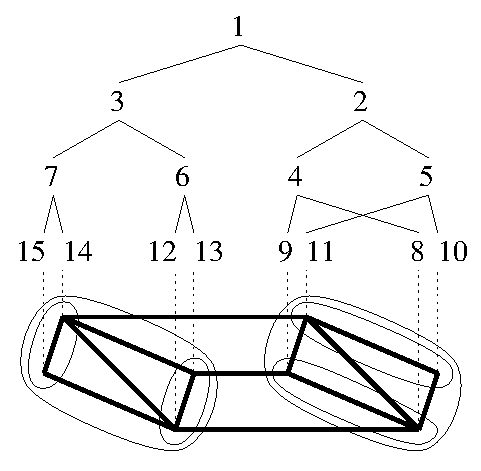
\includegraphics[width=0.7\linewidth]{s_f_d.ps}}
\end{center}
&
\begin{center}
{\renewcommand{\baselinestretch}{1.05}
\footnotesize\tt
\begin{verbatim}
deco 0
8	15
0	1	15
1	1	14
2	1	13
3	1	11
4	1	12
5	1	9
6	1	8
7	1	10
1
2 1
2 1 2
1 1 1 2
3 2 1 1 2
2 2 2 1 1 1
3 2 3 1 2 2 1
\end{verbatim}
}
\end{center}
\end{tabular}
\caption{Target decomposition file for $\UB(2,3)$.
         The terminal numbers associated with every processor define a unique
         recursive bipartitioning of the target graph.}
\label{fig-file-targetdeco}
\end{figure}

The ``\texttt{deco 2}'' format was created so as to represent bigger
target architectures. Indeed, the distance matrix of the
``\texttt{deco 0}'' format is quadratic in the number of target
vertices, which is not scalable and prevents users from representing
target architectures bigger than a few thousand vertices. In the
``\texttt{deco 2}'' architecture, distances are computed using in a
multilevel representation of the target graph, in the form of a family
of coarser graphs. Hence, the more distant the vertices are, the
coarsest is the graph to be used to estimate this
distance~\cite{pellegrini:hal-01671156}. The vertices and edges of
these graphs encode their respective cost of traversal, which becomes
less accurate as coarser graphs are used.

\subsubsection{Algorithmically-coded architecture files}
\label{sec-file-target-algo}

Almost all algorithmically-coded architectures are defined with unity
edge and vertex weights. They start with an abbreviation name of the
architecture, followed by parameters specific to the architecture. The
available built-in architecture definitions are listed below.
\begin{itemize}
\iteme[{\texttt{cmplt} {\it size}}]
Defines a complete graph with $\mathit{size}$ vertices.
Its vertex labels are numbers between $0$ and $\mathit{size} - 1$.
%%
\iteme[{\texttt{cmpltw} {\it size} {\it load$_0$} {\it load$_1$}
\ldots\ {\it load$_{\mathit{size} - 1}$}}]
Defines a weighted complete graph with {\it size\/} vertices.
Its vertex labels are numbers between $0$ and $\mathit{size} - 1$,
and vertices are assigned integer weights in the order in which
these are provided.
%%
\iteme[{\texttt{hcub} $\mathit{dim}$}]
Defines a binary hypercube of dimension $\mathit{dim}$.
Graph vertices are numbered according to the value of the binary
representation of their coordinates in the hypercube.
%%
\iteme[{\texttt{ltleaf}
\parbox[t]{11cm}{$\mathit{levlnbr}$ $\mathit{sizeval}_0$ $\mathit{linkval}_0$
\ldots\ $\mathit{sizeval}_{\mathit{levlnbr}-1}$
$\mathit{linkval}_{\mathit{levlnbr}-1}$
\\
$\mathit{permnbr}$ $\mathit{permval}_0$
\ldots\ $\mathit{permval}_{\mathit{permnbr}-1}$}}]
\label{sec-file-target-ltleaf}
The \texttt{ltleaf} (for ``\textit{labeled tree-leaf}'') architecture is
an extended tree-leaf architecture (\texttt{tleaf}, see below) which
models target topologies where cores are not labeled in increasing
order.
\\
The tree structure of the architecture is described just like for a
regular \texttt{tleaf} architecture. $\mathit{permnbr}$ is the length
of the permutation that is used to label cores, followed by this
number of permutation indices, ranging between $0$ and
$(\mathit{permnbr}-1)$. Figure~\ref{fig-file-targetltleaf} presents an
example of such an architecture.
\\
The permutation array must be of a size that matches level
boundaries. Alternatively, a permutation of size $1$, with only index
$0$ given, represents the identity permutation. In this case, the
regular \texttt{tleaf} architecture can be used.
\begin{figure}[hbt]
\begin{center}
\begin{minipage}[b]{6cm}
{\renewcommand{\baselinestretch}{1.05}
\footnotesize\tt
\begin{verbatim}
ltleaf
3 32 10 2 5 4 1
8 0 2 4 6 1 3 5 7
\end{verbatim}
}\end{minipage}
\end{center}
\caption{Labeled tree-leaf architecture with $3$ levels, representing
a system with $32$ nodes of $2$ quad-core processors. Inter-node
communication costs $10$, inter-processor communication within the
same node costs $5$ and inter-core communication within the same
processor costs $1$. Within a $8$-core node, cores are labeled such
that cores $0$, $2$, $4$ and $6$ are located on the first processor,
while cores $1$, $3$, $5$ and $7$ are located on the second processor.}
\label{fig-file-targetltleaf}
\end{figure}
%%
\iteme[{\texttt{mesh2D} {\it dim$_X$} {\it dim$_Y$}}]
Defines a bidimensional array of {\it dim$_X$} columns by {\it dim$_Y$}
rows. The vertex with coordinates $(\mathit{pos_X},\mathit{pos_Y})$
has label $\mathit{pos_X} + \mathit{pos_Y} \times \mathit{dim_X}$.
%%
\iteme[{\texttt{mesh3D} {\it dim$_X$} {\it dim$_Y$} {\it dim$_Z$}}]
Defines a tridimensional array of {\it dim$_X$} columns by {\it dim$_Y$}
rows by {\it dim$_Z$} levels. The vertex with coordinates
($\mathit{pos_X},\mathit{pos_Y},\mathit{pos_Z}$) has label
$\mathit{pos_X} + \mathit{pos_Y} \mathit{dim_X} + \mathit{pos_Z} \mathit{dim_X} \mathit{dim_Y}$.
%%
\iteme[{\texttt{meshXD} {\it ndims} {\it dim$_0$} {\it dim$_1$} \ldots
{\it dim$_{(ndims - 1)}$}}]
Generalization of the \texttt{mesh2D} and \texttt{mesh3D}
architectures. Defines a \textit{ndims}-dimensional array of
dimensions \textit{dim$_0$}, \textit{dim$_1$} \ldots
\textit{dim$_{ndims - 1}$}. The vertex with coordinates 
($\mathit{pos_0},\mathit{pos_1},\ldots,\mathit{pos_{ndims - 1}}$)
has label $\mathit{pos_0} + \sum_{d=1}^{ndims - 1}\left(\mathit{pos_d} \prod_{d'=0}^{d-1}\mathit{dim_{d'}}\right)$.
%%
\iteme[{\texttt{sub} $\mathit{termnbr}$ $\mathit{termnum}_0$
$\mathit{termnum}_1$ \ldots\ $\mathit{termnum}_{\mathit{termnbr}-1}$
$\mathit{architecture}$}]
Defines a sub-architecture of another \textit{architecture}. The
sub-architecture contains $\mathit{termnbr}$ vertices, which have
ranks $\mathit{termnum}_0$, $\mathit{termnum}_1$,
\ldots\ $\mathit{termnum}_{\mathit{termnbr}-1}$ in the prescribed,
original $\mathit{architecture}$. The original architecture must
comprise at least $\mathit{termnbr}$ vertices, and thus cannot be a
variable-sized architecture. The order in which vertex numbers are
provided defines the part indices that will be used as output
mapping data. For instance, in the example shown in
Figure~\ref{fig-file-targetsub}, source vertices that are assigned to
vertex $3$ of the sub-architecture are in fact assigned to vertex $5$
of the original, 2D mesh architecture, according to its canonical
numbering.
\begin{figure}[hbt]
\begin{tabular}{p{0.69\linewidth}@{}p{0.29\linewidth}}
\begin{center}
\parbox[t]{0.9\linewidth}{\vspace{0pt}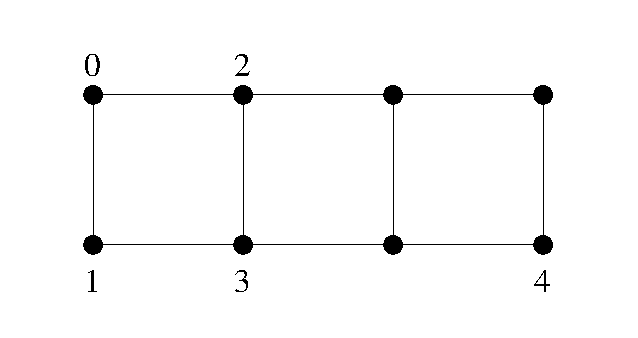
\includegraphics[width=0.7\linewidth]{m42_a1}}
\end{center}
&
\begin{center}
{\renewcommand{\baselinestretch}{1.05}
\footnotesize\tt
\begin{verbatim}


sub
5 0 4 1 5 7
mesh2D 4 2
\end{verbatim}
}
\end{center}
\end{tabular}
\caption{Sub-architecture of a 4x2 \texttt{mesh2D} 2D grid
  architecture. The sub-architecture comprises $5$ vertices, numbered
  from $0$ to $4$, which correspond to vertices $0$, $4$, $1$, $5$ and
  $7$ of the original architecture, respectively.}
\label{fig-file-targetsub}
\end{figure}
%%
\iteme[{\texttt{tleaf} $\mathit{levlnbr}$ $\mathit{sizeval}_0$
$\mathit{linkval}_0$ \ldots\ $\mathit{sizeval}_{\mathit{levlnbr}-1}$
$\mathit{linkval}_{\mathit{levlnbr}-1}$}]
Defines a hierarchical, tree-shaped, architecture with $\mathit{levlnbr}$
levels and $\sum_{i=0}^{\mathit{levlnbr}-1}\mathit{sizeval}_i$
leaf vertices. This topology is used to model hierarchical NUMA or NUIOA
machines. The mapping is only computed with respect to the leaf
vertices, which represent processing elements, while the upper levels of
the tree model interconnection networks (intra-chip buses, inter-chip
interconnection networks, network routers, etc.), as exemplified in
Figure~\ref{fig-graf-treeleaf}. The communication cost between two
nodes is the cost of the highest common ancestor level.
\begin{figure}[hbt]
\begin{tabular}{p{0.69\linewidth}@{}p{0.29\linewidth}}
\begin{center}
\parbox[t]{0.9\linewidth}{\vspace{0pt}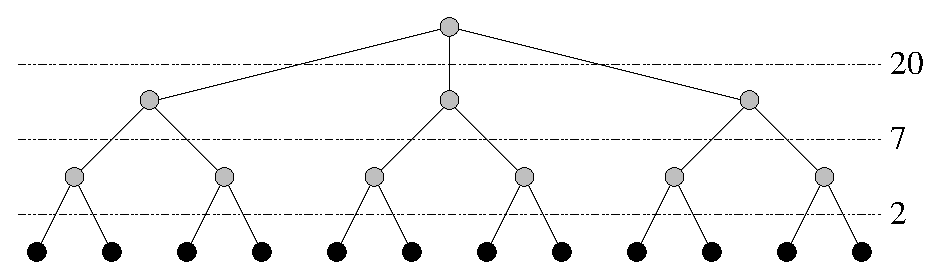
\includegraphics[width=0.95\linewidth]{s_f_lea.eps}}
\end{center}
&
\begin{center}
{\renewcommand{\baselinestretch}{1.05}
\footnotesize\tt
\begin{verbatim}


tleaf
3 3 20 2 7 2 2
\end{verbatim}
}
\end{center}
\end{tabular}
\caption{A ``tree-leaf'' graph with three levels. Processors are drawn
in black and routers in grey. It has $3$ levels, the first level has
$3$ sons and a traversal cost of $20$, the second level has $2$ sons
and a traversal cost of $7$, and the third level has also $2$ sons and
a traversal cost of $2$.}
\label{fig-graf-treeleaf}
\end{figure}
%%
\iteme[{\texttt{torus2D} {\it dim$_X$} {\it dim$_Y$}}]
Defines a bidimensional array of {\it dim$_X$} columns by {\it dim$_Y$}
rows, with wraparound edges.
The vertex with coordinates $(\mathit{pos_X},\mathit{pos_Y})$ has label
$\mathit{pos_X} + \mathit{pos_Y} \times \mathit{dim_X}$.
%%
\iteme[{\texttt{torus3D} {\it dim$_X$} {\it dim$_Y$} {\it dim$_Z$}}]
Defines a tridimensional array of {\it dim$_X$} columns by {\it dim$_Y$}
rows by {\it dim$_Z$} levels, with wraparound edges. The vertex with
coordinates $(\mathit{pos_X},\mathit{pos_Y},\mathit{pos_Z})$ has
label
$\mathit{pos_X} + \mathit{pos_Y} \mathit{dim_X} + \mathit{pos_Z} \mathit{dim_X} \mathit{dim_Y}$.
%%
\iteme[{\texttt{torusXD} {\it ndims} {\it dim$_0$} {\it dim$_1$} \ldots
{\it dim$_{ndims - 1}$}}]
Generalization of the \texttt{torus2D} and \texttt{torus3D}
architectures. Defines a \textit{ndims}-dimensional torus of
dimensions \textit{dim$_0$}, \textit{dim$_1$} \ldots
\textit{dim$_{ndims - 1}$}. The vertex with coordinates 
($\mathit{pos_0},\mathit{pos_1},\ldots,\mathit{pos_{(ndims - 1)}}$)
has label $\mathit{pos_0} + \sum_{d=1}^{ndims - 1}\left(\mathit{pos_d} \prod_{d'=0}^{d-1}\mathit{dim_{d'}}\right)$.
\end{itemize}

\subsubsection{Variable-sized architecture files}
\label{sec-file-target-variable}
\index{Clustering}

Variable-sized architectures are a class of algorithmically-coded
architectures the size of which is not defined {\it a priori}. Domains
of these target architectures can always be bipartitioned, again and
again (until integer overflow occurs in domain indices). These
architectures are used to perform graph clustering (see
Sections~\ref{sec-prog-gmap} and~\ref{sec-lib-func-graphmap}),
using a specifically tailored graph mapping strategy (see for instance
Section~\ref{sec-lib-func-stratgraphclusterbuild}).

As for fixed-size algorithmically-coded architectures, they start with
an abbreviation name of the architecture, followed by parameters
specific to the architecture. The available built-in variable-sized
architecture definitions are listed below.
\begin{itemize}
\iteme[{\texttt{varcmplt}}]
Defines a variable-sized complete graph. Domains are labeled such
that the first domain is labeled $1$, and the two subdomains of
any domain $i$ are labeled $2i$ and $2i + 1$. The distance between
any two subdomains $i$ and $j$ is $0$ if $i=j$ and $1$ else.
\iteme[{\texttt{varhcub}}]
Defines a variable-sized hypercube. Domains are labeled such that
the first domain is labeled $1$, and the two subdomains of any domain
$i$ are labeled $2i$ and $2i + 1$. The distance between any two
domains is the Hamming distance between the common bits of the two
domains, plus half of the absolute difference between the levels of
the two domains, this latter term modeling the average distance on
unknown bits.
For instance, the distance between subdomain $9=1001_B$, of level $3$
(since its leftmost $1$ has been shifted left thrice), and subdomain
$53=110101_B$, of level $5$ (since its leftmost $1$ has been shifted
left five times), is equal to $2$: it is $1$, which is the number of
bits which differ between $1101_B$ (that is, $53=110101_B$ shifted
rightwards twice) and $1001_B$, plus $1$, which is half of the
absolute difference between $5$ and $3$.
\end{itemize}

\subsection{Mapping files}
\label{sec-file-map}

Mapping files, which usually end in ``\texttt{\@.map}'', contain the
result of the mapping of source graphs onto target architectures. They
associate a vertex of the target graph with every vertex of the source
graph.

Mapping files begin with the number of mapping lines which they contain,
followed by that many mapping lines.
Each mapping line holds a mapping pair, made of two integer numbers
which are the label of a source graph vertex and the label
of the target graph vertex onto which it is mapped.
Mapping pairs can be stored in any order in the file; however, labels of
source graph vertices must be all different.
For example, Figure~\ref{fig-file-mapping} shows the result obtained when
mapping the source graph of Figure~\ref{fig-file-sgraph} onto the target
architecture of Figure~\ref{fig-file-targetdeco}.
This one-to-one embedding of $\HY(3)$ into $\UB(2,3)$ has dilation~$1$,
except for one hypercube edge which has dilation~$3$.
\begin{figure}[hbt]
\begin{center}
\begin{minipage}{3cm}
{\renewcommand{\baselinestretch}{1.05}
\footnotesize\tt
\begin{verbatim}
8
0       1
1       3
2       2
3       5
4       0
5       7
6       4
7       6
\end{verbatim}
}\end{minipage}
\end{center}
\caption{Mapping file obtained when mapping the hypercube source graph of
         Figure~\protect\ref{fig-file-sgraph} onto the binary de~Bruijn
         architecture of Figure~\protect\ref{fig-file-targetdeco}.}
\label{fig-file-mapping}
\end{figure}

Mapping files are also used on output of the block orderer to
represent the allocation of the vertices of the original graph to the
column blocks associated with the ordering. In this case, column blocks
are labeled in ascending order, such that the number of a block is
always greater than the ones of its predecessors in the elimination
process, that is, its leaves in the elimination tree.

\subsection{Ordering files}
\label{sec-file-ord}

Ordering files, which usually end in ``\texttt{\@.ord}'', contain the
result of the ordering of source graphs or meshes that represent
sparse matrices. They associate a number with every vertex of the
source graph or mesh.

The structure of ordering files is analogous to the one of mapping
files; they differ only by the meaning of their data.

Ordering files begin with the number of ordering lines which they
contain, that is the number of vertices in the source graph or the
number of nodes in the source mesh, followed by that many ordering
lines. Each ordering line holds an ordering pair, made of two integer
numbers which are the label of a source graph or mesh vertex and its
rank in the ordering. Ranks range from the base value of the graph or
mesh (\texttt{baseval}) to the base value plus the number of vertices
(resp\@. nodes), minus one ($\mbox{\texttt{baseval}} +
\mbox{\texttt{vertnbr}} - 1$ for graphs, and $\mbox{\texttt{baseval}}
+ \mbox{\texttt{vnodnbr}} - 1$ for meshes).  Ordering pairs can be
stored in any order in the file; however, indices of source vertices
must be all different.

For example, Figure~\ref{fig-file-ordering} shows the result obtained
when reordering the source graph of Figure~\ref{fig-file-sgraph}.
\begin{figure}[hbt]
\begin{center}
\begin{minipage}{3cm}
{\renewcommand{\baselinestretch}{1.05}
\footnotesize\tt
\begin{verbatim}
8
0       6
1       3
2       2
3       7
4       1
5       5
6       4
7       0
\end{verbatim}
}\end{minipage}
\end{center}
\caption{Ordering file obtained when reordering the hypercube graph of
Figure~\protect\ref{fig-file-sgraph}.}
\label{fig-file-ordering}
\end{figure}

The advantage of having both graph and mesh orderings start from
\texttt{baseval} (and not \texttt{vnodbas} in the case of meshes) is
that an ordering computed on the nodal graph of some mesh has the same
structure as an ordering computed from the native mesh structure,
allowing for greater modularity. However, in memory, permutation
indices for meshes are numbered from \texttt{vnodbas} to
$\mbox{\texttt{vnodbas}} + \mbox{\texttt{vnodnbr}} - 1$.

\subsection{Vertex list files}

Vertex lists are used by programs that select vertices from graphs.

Vertex lists are coded as lists of integer numbers.
The first integer is the number of vertices in the list and
the other integers are the labels of the selected vertices, given in
any order.
For example, Figure~\ref{fig-file-vertex} shows the list made from
three vertices of labels $2$, $45$, and $7$.
\begin{figure}[hbt]
\begin{center}
\begin{minipage}{3cm}
{\renewcommand{\baselinestretch}{1.05}
 \footnotesize \tt \begin{verbatim}
3   2   45   7
\end{verbatim}}
\end{minipage}
\end{center}
\caption{Example of vertex list with three vertices of labels~$2$, $45$, and~$7$.}
\label{fig-file-vertex}
\end{figure}
